\chapter{Work Done}

\section{Progress Made By Project Midterm}

\subsection{Image Slicing}
The data drawn from the Kinect is in 2D depth image format. Which is a grey-scale image where the distances of all points are represented by a single value. The closer the surface the brighter it shows on the image.

The problem with the structure of the raw data is, when the objects are very close or very similar in height the differences corresponding to respective surfaces become too subtle  to extract object from. In those cases the data raises false positives.

To alleviate this, we used image slicing. Image slicing is an image processing technique where pixel values outside certain regions are reduced to zero.

As shown in figure \ref{fig:label31}, by fading all areas outside a certain region to black objects within that region are depicted with much more contrast since the dynamic range is focussed on a much smaller area. 

With this false negative are removed but the calibration is of utmost importance. If the regions near and far borders are not determined properly desired objects are lost completely.
\subsection{Blob Tracking}
As the main aim of the project is object tracking, we directed most of our effort to this area.

Once the depth image from the Kinect is cleaned up we extract the contours of the image and encapsulate them in rectangles which are inner representations of the captured objects as shown in figure \ref{fig:label31}.

This part is implemented with the help of OpenCv libraries which provides helper functions for both jobs: extracting contours and marking them.
\begin{figure}[htb]
\centering
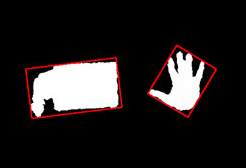
\includegraphics[scale=2]{./tracker} % e.g. insert ./image for image.png in the working directory, adjust scale as necessary
\caption{Sliced image with objects marked}
\label{fig:label31} % insert suitable label, this is used to refer to a fig from within the text as shown above
\end{figure}
\subsection{User Interface}
As a prototype a UI is built to track objects with Kinect. This program while recording the processed video, slices the image, isolates the objects. 
\begin{figure}[htb]
\centering
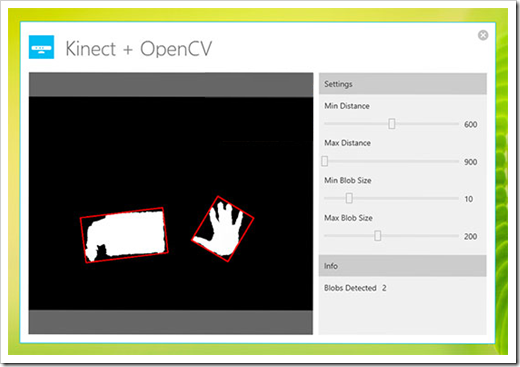
\includegraphics[scale=1]{./UI} % e.g. insert ./image for image.png in the working directory, adjust scale as necessary
\caption{Prototype User Interface}
\label{fig:label32} % insert suitable label, this is used to refer to a fig from within the text as shown above
\end{figure}

As shown in figure \ref{fig:label31}, the relevant UI element are the sliders to calibrate far and near borders for the slicer and max/min blob sizes.As of nbow calibration of these variables are done by hand and are very important to properly isolate objects to be tracked.
\subsection{Multi-Threading}
For performance purposes we chose to separate video record and object tracking functionality to their ow threads. this significantly improved performance as these functions were no longer impeded by each other and the UI load.

